% =====================================================================
% INFORME: Detección de Anomalías DNS con TinyML en ESP32
% Compilar con: pdflatex -shell-escape informe.tex
% =====================================================================
\documentclass[12pt,a4paper]{article}

% ---- Paquetes ----
\usepackage[utf8]{inputenc}
\usepackage[spanish]{babel}
\usepackage{amsmath,amssymb}
\usepackage{graphicx}
\usepackage{booktabs}
\usepackage{array}
\usepackage{xcolor}
\usepackage{listings}
\usepackage{hyperref}
\usepackage{geometry}
\usepackage{caption}
\usepackage{subcaption}
\usepackage{float}
\usepackage{fancyhdr}
\usepackage{setspace}
\usepackage{enumitem}
\usepackage{tabularx}

\geometry{left=2.5cm,right=2.5cm,top=2.5cm,bottom=2.5cm}
\onehalfspacing

% ---- Configuración de listings (código) ----
\lstset{
    basicstyle=\footnotesize\ttfamily,
    numbers=left,
    numberstyle=\tiny,
    stepnumber=1,
    frame=single,
    breaklines=true,
    tabsize=4,
    captionpos=b,
    backgroundcolor=\color{gray!5},
    rulecolor=\color{gray!30},
    keywordstyle=\color{blue}\bfseries,
    commentstyle=\color{green!50!black},
    stringstyle=\color{red}
}

% INSTRUCCIONES PARA OVERLEAF:
% 1. Crear proyecto nuevo en Overleaf
% 2. Pegar este contenido en informe.tex
% 3. Crear carpeta "graficas/" y subir todos los PNG de EC2/graficas/
% 4. Crear carpeta "src/" y subir main.cpp y modelo.h
% 5. Compilar con pdflatex (o latexmk)

% ---- Portada ----
\title{\Huge \textbf{Detección de Anomalías DNS\\ con TinyML en ESP32}}
\author{
    Oscar David \\
    \texttt{Ingeniería en Sistemas Computacionales}
    \vspace{1cm}
}
\date{\today}

\begin{document}
\maketitle
\thispagestyle{empty}
\newpage

% ---- Índice ----
\tableofcontents
\newpage

% =====================================================================
% a) ESTADO DEL ARTE
% =====================================================================
\section{Estado del Arte}
\label{sec:estado}

El uso de TinyML para detección de intrusiones y anomalías en redes IoT es un área de investigación activa. A continuación se revisan 5 trabajos relevantes:

\subsection{TinyML para detección de intrusiones en cortes de red 5G}
\label{sec:paper5}

Patnaik et al.~\cite{patnaik2026tinyml} proponen un detector de intrusiones ligero para cortes de red 5G utilizando regresión logística sobre estadísticas de flujo extraídas del dataset 5G-NIDD. Aplican poda por importancia de características y cuantización INT8, logrando una latencia de inferencia menor a 1 ms. El énfasis está en la evaluación libre de fuga de datos (leakage-free), separando cronológicamente tráfico de entrenamiento y prueba. Los resultados son estables para tráfico eMBB y mMTC, aunque limitados para URLLC por falta de representación en el dataset.

\subsection{Modelo TinyML basado en stacking optimizado para detección de ataques en IoT}
\label{sec:paper1}

Un estudio publicado en PLOS One~\cite{stacking2025tinyml} presenta un modelo de stacking que combina árboles de decisión ligeros y redes neuronales pequeñas, usando Regresión Logística como metaclasificador. Evaluado en el dataset ToN-IoT, alcanza 99.98\% de precisión, 0.12 ms de latencia y 0.01 mW de consumo. Utiliza Random Forest para selección de características y demuestra que los ensembles TinyML superan a modelos individuales en entornos IoT con recursos limitados.

\subsection{Detección de intrusiones eficiente con ML en ESP32}
\label{sec:paper2}

Este trabajo (de próxima publicación) se enfoca específicamente en modelos de Machine Learning ejecutándose en ESP32 para detección de intrusiones. Explora la viabilidad de clasificadores como árboles de decisión, Random Forest y MLPs en microcontroladores, comparando accuracy, tamaño de modelo y latencia. Es el antecedente más directo de nuestro proyecto.

\subsection{TinyML federado y eficiente en energía para detección de anomalías sobre LoRaWAN}
\label{sec:paper3}

Anand y Borisagar~\cite{anand2026energy} implementan detección de anomalías por vibraciones con TinyML en ESP32 usando sensor MPU6050 y transmisión LoRa. El sistema procesa datos localmente y solo envía eventos anómalos, reduciendo el consumo energético. Incorporan un concepto de aprendizaje federado donde múltiples nodos comparten información resumida en lugar de datos crudos. Incluyen un dashboard en Python para visualización en tiempo real.

\subsection{Detección de intrusiones ligera y eficiente en energía para IIoT con TinyML y Edge AI}
\label{sec:paper4}

Nassef et al.~\cite{nassef2026lightweight} proponen un framework híbrido GAT-BiGRU optimizado con Grey Wolf Optimizer y Federated Learning para detección de intrusiones en IIoT. Alcanza 95\% de precisión en datasets EDGE-IIoTset, CICIoT2023 y RT-IoT2022. Incluye un módulo XAI basado en atención de GAT para interpretabilidad. Si bien el modelo es más complejo que un árbol de decisión, demuestra la viabilidad de TinyML en entornos industriales.

\subsection{Resumen comparativo}
\label{sec:resumen}

La Tabla~\ref{tab:estado} resume los trabajos revisados.

\begin{table}[H]
\centering
\caption{Comparativa de trabajos relacionados}
\label{tab:estado}
\small
\begin{tabularx}{\textwidth}{Xccc}
\toprule
\textbf{Trabajo} & \textbf{Modelo} & \textbf{Precisión} & \textbf{Latencia} \\
\midrule
Patnaik et al.~(2026) & Regresión Logística + cuantización INT8 & -- & $<$1 ms \\
Stacking-based (2025) & DT + NN + LR (stacking) & 99.98\% & 0.12 ms \\
ML en ESP32 & DT/RF/MLP (TinyML) & -- & -- \\
Anand et al.~(2026) & TinyML (anomalías) + LoRa & -- & -- \\
Nassef et al.~(2026) & GAT-BiGRU + GWO + FL & 95\% & 120-180 ms \\
\midrule
\textbf{Este trabajo} & \textbf{DecisionTree (13 nodos)} & \textbf{64.86\%} & \textbf{$\ll$1 ms} \\
\bottomrule
\end{tabularx}
\end{table}

% =====================================================================
% b) PROBLEMA: OBJETIVOS E HIPÓTESIS
% =====================================================================
\section{Problema, Objetivos e Hipótesis}
\label{sec:problema}

\subsection{Planteamiento del problema}
\label{sec:problema-planteamiento}

Las redes WiFi domésticas y de pequeña oficina carecen de sistemas de detección de intrusiones debido al costo y complejidad de las soluciones tradicionales. Los dispositivos IoT y smartphones generan tráfico DNS que puede revelar patrones de comportamiento anómalos (malware, fuga de datos, C\&C). Sin embargo, no existe una solución ligera que pueda ejecutarse en un ESP32 actuando como gateway.

\subsection{Objetivo general}
\label{sec:objetivo-general}

Diseñar e implementar un sistema de detección de anomalías DNS en tiempo real utilizando TinyML en un ESP32, capaz de clasificar el tráfico en background, foreground y sospechoso, y visualizar los resultados en un dashboard web.

\subsection{Objetivos específicos}
\label{sec:objetivos-especificos}

\begin{enumerate}[label=OE\arabic*:]
    \item Implementar un forwarder DNS en ESP32 que capture y reenvíe consultas DNS.
    \item Extraer características estadísticas por ventanas de tiempo (cantidad, dominios únicos, dominios nuevos).
    \item Entrenar un árbol de decisión TinyML con datos etiquetados manualmente.
    \item Integrar el modelo en el firmware del ESP32 para clasificación en tiempo real.
    \item Enviar los resultados a un servidor EC2 para visualización en dashboard WebSocket.
    \item Validar el prototipo con tráfico real de navegación.
\end{enumerate}

\subsection{Hipótesis}
\label{sec:hipotesis}

\textbf{H1:} Las consultas DNS (cantidad, dominios únicos y dominios nuevos por ventana de 3 segundos) contienen suficiente información para distinguir entre tráfico de fondo, navegación activa y actividad sospechosa.

\textbf{H2:} Un árbol de decisión de profundidad limitada ($\leq$5) puede ejecutarse en un ESP32 con latencia insignificante ($\ll$1 ms) y consumir menos del 1\% de la memoria flash disponible.

\textbf{H3:} El sistema puede clasificar ventanas de tráfico en tiempo real con una precisión superior al 60\% usando solo 3 features.

% =====================================================================
% c) ARQUITECTURA, CIRCUITO Y FLUJO
% =====================================================================
\section{Arquitectura, Circuito y Flujo}
\label{sec:arquitectura}

\subsection{Arquitectura del sistema}
\label{sec:arquitectura-sistema}

La Figura~\ref{fig:arquitectura} muestra la arquitectura general del sistema.

\begin{figure}[H]
\centering
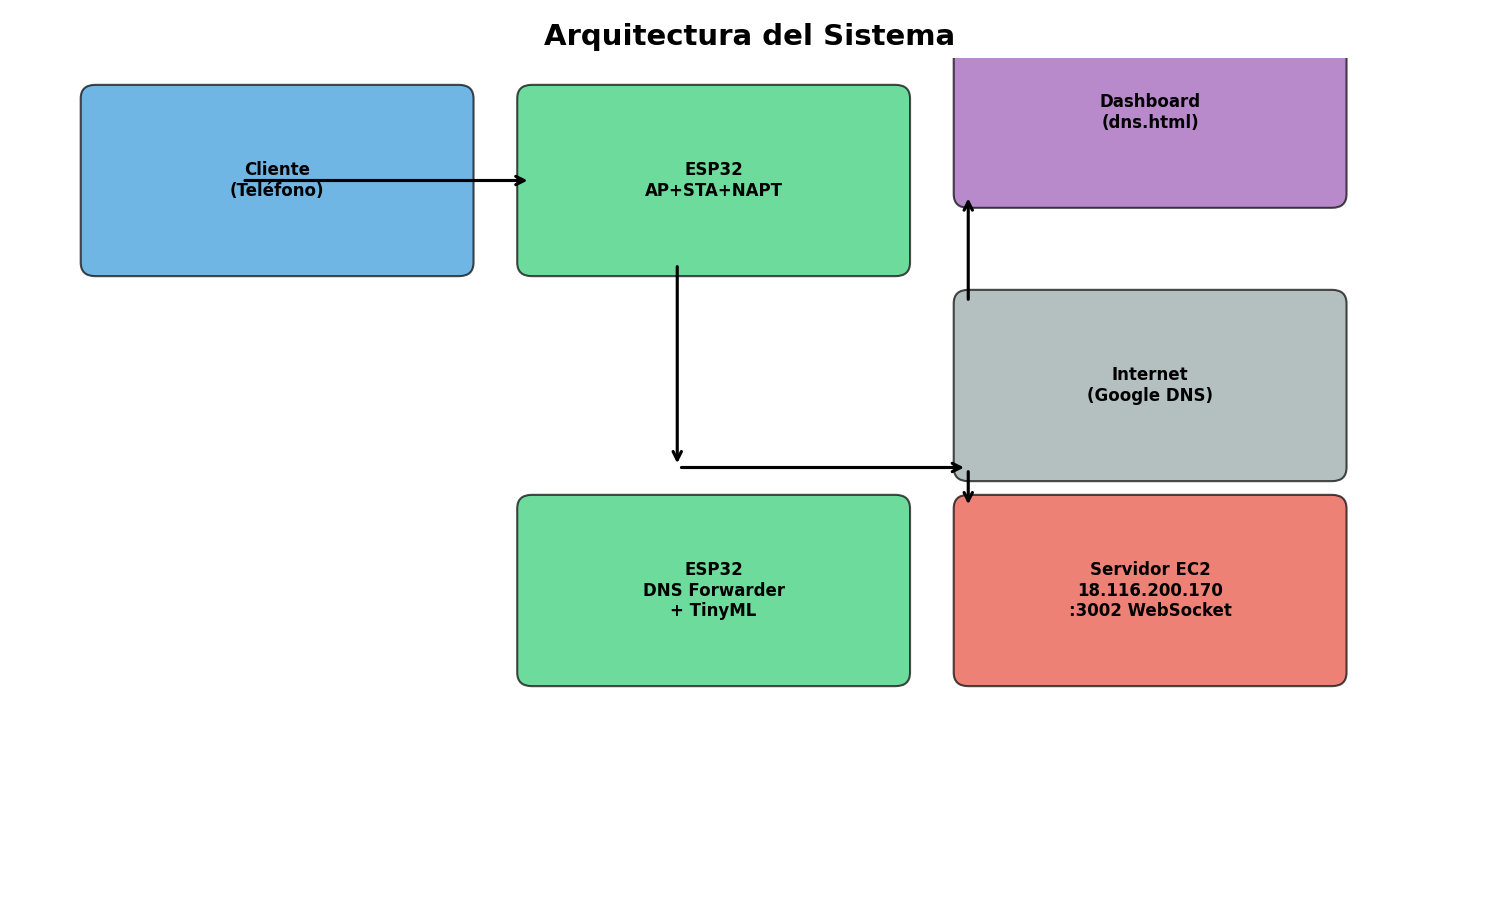
\includegraphics[width=\textwidth]{graficas/arquitectura.png}
\caption{Arquitectura del sistema de detección de anomalías DNS}
\label{fig:arquitectura}
\end{figure}

El sistema consta de los siguientes componentes:

\begin{enumerate}
    \item \textbf{ESP32 (Gateway WiFi):} Actúa en modo AP+STA. Crea una red WiFi local (ESP32-Monitor) a la que se conectan los dispositivos cliente (ej. teléfono). Simultáneamente se conecta a internet via STA. Habilita NAPT para compartir la conexión.
    \item \textbf{Forwarder DNS:} Escucha en puerto 53, captura consultas DNS entrantes, extrae el nombre de dominio, actualiza contadores estadísticos y reenvía la consulta a Google DNS (8.8.8.8).
    \item \textbf{Motor de ventanas:} Cada 3 segundos cierra una ventana, calcula 3 features (dns\_qty, dns\_unique, dns\_new), y las pasa al clasificador TinyML.
    \item \textbf{Clasificador TinyML:} Árbol de decisión de 13 nodos integrado en el firmware. Clasifica cada ventana en background (0), foreground (1) o sospechoso (2).
    \item \textbf{Servidor EC2:} Recibe los datos via HTTP POST en el puerto 3002. Un WebSocket broker (csi\_ws.py) los retransmite a todos los clientes conectados.
    \item \textbf{Dashboard web:} Página HTML (dns.html) que se conecta via WebSocket y muestra en tiempo real la clasificación, métricas y gráficos históricos.
\end{enumerate}

\subsection{Circuito}
\label{sec:circuito}

El circuito es mínimo: solo el ESP32 conectado por USB a una fuente de alimentación (5V). No se requieren sensores externos. La Figura~\ref{fig:circuito} muestra el diagrama.

\begin{figure}[H]
\centering
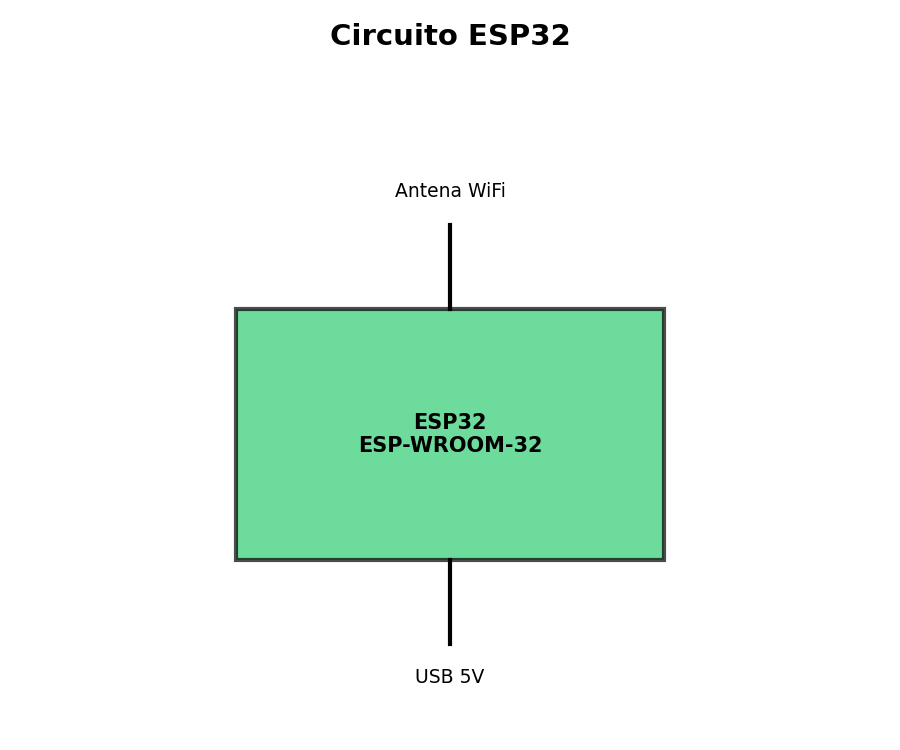
\includegraphics[width=0.6\textwidth]{graficas/circuito.png}
\caption{Diagrama de conexión del ESP32}
\label{fig:circuito}
\end{figure}

\begin{table}[H]
\centering
\caption{Componentes utilizados}
\label{tab:componentes}
\begin{tabular}{ll}
\toprule
\textbf{Componente} & \textbf{Especificación} \\
\midrule
Microcontrolador & ESP-WROOM-32 (Xtensa LX6 dual-core @ 240MHz) \\
Flash & 4 MB \\
RAM & 520 KB SRAM \\
Conectividad & WiFi 802.11 b/g/n (2.4 GHz) \\
Alimentación & 5V USB \\
\bottomrule
\end{tabular}
\end{table}

\subsection{Flujo de datos}
\label{sec:flujo}

\begin{enumerate}
    \item El ESP32 inicia en modo AP+STA y habilita NAPT.
    \item Los clientes se conectan al AP y realizan consultas DNS.
    \item El forwarder captura cada consulta, extrae el dominio y actualiza contadores.
    \item Cada 3 segundos se cierra la ventana y se calculan las 3 features.
    \item El árbol de decisión clasifica la ventana.
    \item Los resultados se imprimen por Serial y se envían via HTTP POST a EC2.
    \item El servidor EC2 recibe el POST y lo retransmite a todos los WebSocket clients.
    \item El dashboard web actualiza los gráficos en tiempo real.
\end{enumerate}

% =====================================================================
% d) DATOS ORIGINALES / DEPURADOS
% =====================================================================
\section{Datos Originales y Depurados}
\label{sec:datos}

\subsection{Captura de datos}
\label{sec:captura}

Los datos se capturaron utilizando el script \texttt{capturar.py} que se comunica con el ESP32 via Serial. Durante la captura, se realizaron 3 fases:

\begin{itemize}
    \item \textbf{Fase 1 (background):} El teléfono conectado al AP del ESP32 sin navegación activa. Se etiquetó cada ventana presionando 'b' en el monitor serie.
    \item \textbf{Fase 2 (foreground):} Navegación activa (YouTube, Google, redes sociales). Se etiquetó con 'f'.
    \item \textbf{Fase 3 (sospechoso):} Se forzaron picos de consultas DNS mediante herramientas de red. Se etiquetó con 's'.
\end{itemize}

Se capturaron 124 ventanas en total, generando el archivo \texttt{datos\_crudos.txt}. Cada línea tiene el formato:

\begin{lstlisting}[frame=none,breaklines=false]
[W] dns_qty=4 unique=2 new=1 anom=0.0 label=foreground pred=fg
\end{lstlisting}

\subsection{Dataset depurado}
\label{sec:dataset}

El script \texttt{procesar.py} convierte \texttt{datos\_crudos.txt} en \texttt{dataset.csv}, con las columnas:

\begin{itemize}
    \item \texttt{dns\_qty}: consultas DNS en la ventana (3s)
    \item \texttt{dns\_unique}: dominios distintos en la ventana
    \item \texttt{dns\_new}: dominios nunca antes vistos globalmente
    \item \texttt{label}: etiqueta textual (background, foreground, sospechoso)
    \item \texttt{y}: clase numérica (0, 1, 2)
\end{itemize}

Se eliminaron ventanas con label ``unlabeled'' y la primera ventana de calentamiento, resultando en 123 filas válidas. La Tabla~\ref{tab:distribucion} muestra la distribución.

\begin{table}[H]
\centering
\caption{Distribución de clases en el dataset}
\label{tab:distribucion}
\begin{tabular}{lrr}
\toprule
\textbf{Clase} & \textbf{Ventanas} & \textbf{Porcentaje} \\
\midrule
Background (0)    & 4    & 3.25\% \\
Foreground (1)    & 52   & 42.28\% \\
Sospechoso (2)    & 67   & 54.47\% \\
\midrule
Total             & 123  & 100\% \\
\bottomrule
\end{tabular}
\end{table}

\begin{figure}[H]
\centering
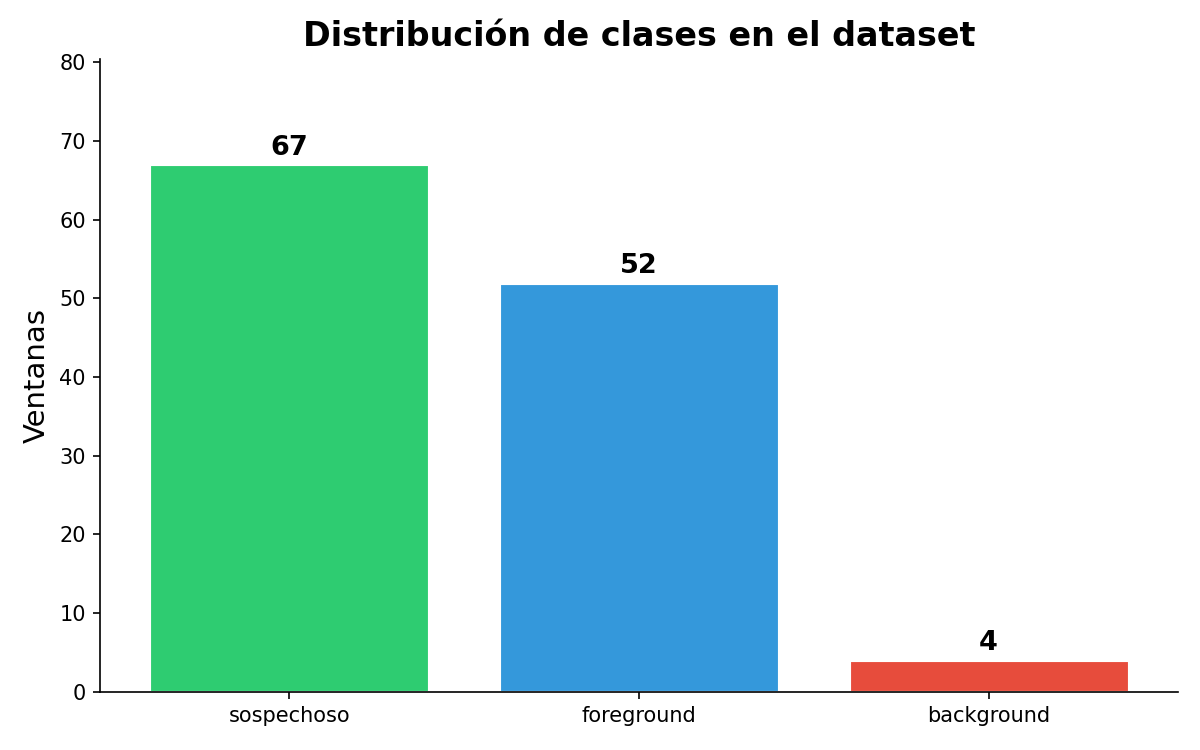
\includegraphics[width=0.75\textwidth]{graficas/distribucion_clases.png}
\caption{Distribución de clases en el dataset}
\label{fig:distribucion}
\end{figure}

\subsection{Análisis exploratorio}
\label{sec:exploratorio}

Las 3 features presentan los siguientes rangos:

\begin{itemize}
    \item \texttt{dns\_qty}: 1--28 consultas por ventana
    \item \texttt{dns\_unique}: 1--20 dominios distintos
    \item \texttt{dns\_new}: 0--14 dominios nuevos
\end{itemize}

Las ventanas de background tienen valores bajos (1--4 consultas), mientras que las sospechosas alcanzan picos de hasta 28 consultas con muchos dominios nuevos.

% =====================================================================
% e) CÓDIGO COMENTADO DEL ESP32
% =====================================================================
\section{Código Comentado del ESP32}
\label{sec:codigo}

\subsection{main.cpp}
\label{sec:main-cpp}

El firmware principal se muestra en el Listado~\ref{lst:main}. Las partes más relevantes son:

\begin{itemize}
    \item \textbf{Forwarder DNS (líneas 122--168):} Captura consultas en puerto 53, extrae el nombre de dominio, actualiza contadores y reenvía a 8.8.8.8.
    \item \textbf{Ventanas (líneas 194--227):} Cada 3s se procesan las estadísticas, se calcula el score de anomalía y se clasifica con TinyML.
    \item \textbf{POST a EC2 (líneas 173--189):} Envía JSON con las features, score de anomalía y predicción.
    \item \textbf{Setup (líneas 232--262):} Inicializa WiFi en modo AP+STA y habilita NAPT.
\end{itemize}

\lstinputlisting[language=C++,caption={main.cpp -- Firmware principal},label={lst:main}]{src/main.cpp}

\subsection{modelo.h}
\label{sec:modelo-h}

El árbol de decisión se muestra en el Listado~\ref{lst:modelo}. Consta de 13 nodos con umbrales escalados $\times 100$ para usar aritmética de enteros.

\lstinputlisting[language=C++,caption={modelo.h -- Árbol de decisión TinyML},label={lst:modelo}]{src/modelo.h}

% =====================================================================
% f) RESULTADOS: MÉTRICAS Y GRÁFICOS
% =====================================================================
\section{Resultados}
\label{sec:resultados}

\subsection{Métricas de clasificación}
\label{sec:metricas}

Se entrenó un árbol de decisión con los siguientes hiperparámetros:
\begin{itemize}
    \item Profundidad máxima: 5
    \item Mínimo de muestras por hoja: 3
    \item Class weight: balanced
\end{itemize}

Se utilizó validación cruzada estratificada de 5 folds y una partición train/test 70/30.

\begin{table}[H]
\centering
\caption{Métricas de clasificación por clase}
\label{tab:metricas}
\begin{tabular}{lcccc}
\toprule
\textbf{Clase} & \textbf{Precisión} & \textbf{Recall} & \textbf{F1-score} & \textbf{Muestras} \\
\midrule
Background  & 0.2000 & 1.0000 & 0.3333 & 1  \\
Foreground  & 0.6667 & 0.3750 & 0.4800 & 16 \\
Sospechoso  & 0.7391 & 0.8500 & 0.7907 & 20 \\
\midrule
Accuracy    &       &        & 0.6486 & 37 \\
Macro avg   & 0.5353 & 0.7417 & 0.5347 &    \\
\bottomrule
\end{tabular}
\end{table}

La precisión general en test es del \textbf{64.86\%}, con un accuracy promedio en validación cruzada de \textbf{62.60\% $\pm$ 5.89\%}.

\subsection{Matriz de confusión}
\label{sec:matriz}

\begin{figure}[H]
\centering
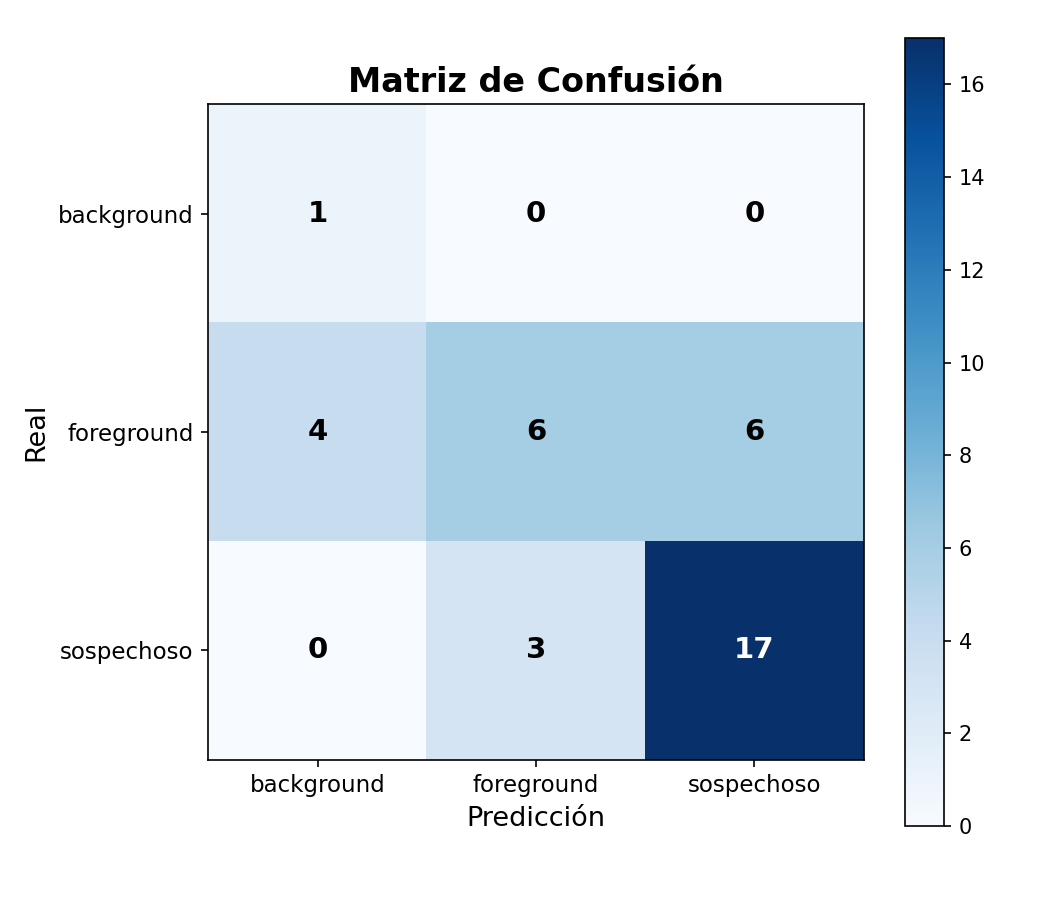
\includegraphics[width=0.6\textwidth]{graficas/confusion_matrix.png}
\caption{Matriz de confusión en el conjunto de test}
\label{fig:confusion}
\end{figure}

La clase \texttt{sospechoso} es la mejor clasificada (17/20 correctas), mientras que \texttt{foreground} tiende a confundirse con \texttt{sospechoso} (6 falsos negativos). La clase \texttt{background} tiene solo 1 muestra en test, lo que limita la significancia estadística.

\subsection{Importancia de características}
\label{sec:importancia}

\begin{figure}[H]
\centering
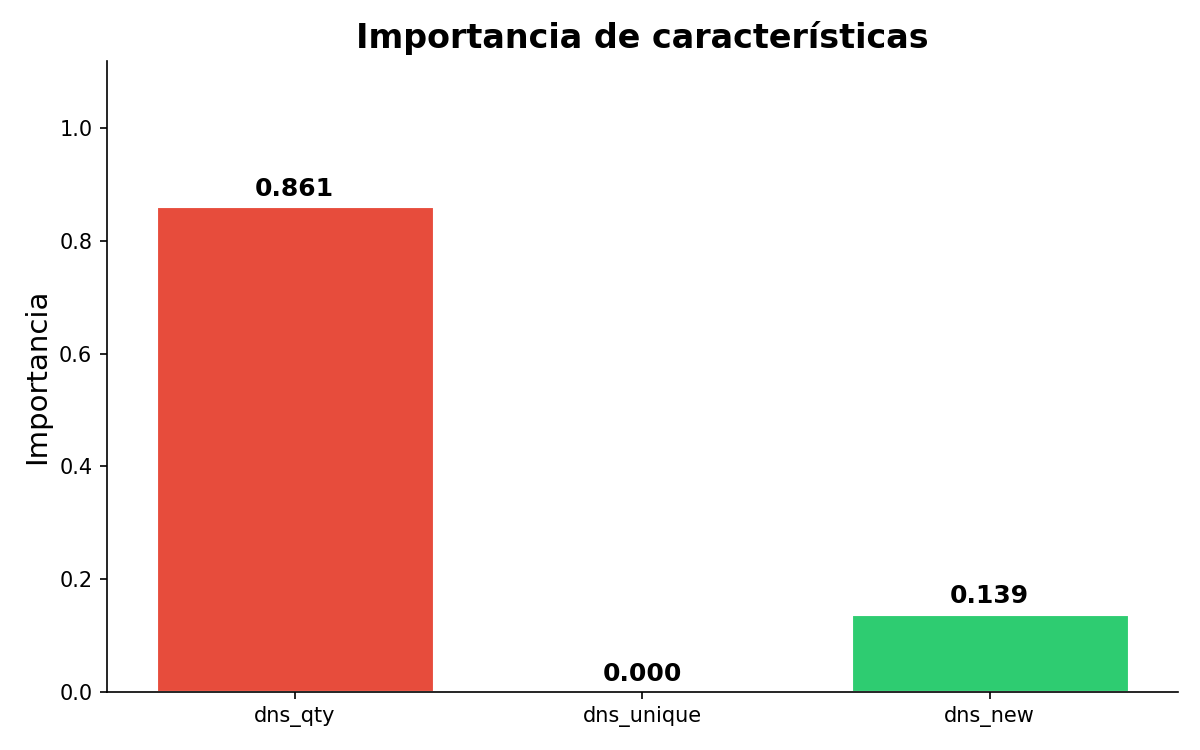
\includegraphics[width=0.7\textwidth]{graficas/feature_importance.png}
\caption{Importancia de características en el árbol de decisión}
\label{fig:importancia}
\end{figure}

La característica \texttt{dns\_qty} (cantidad de consultas) domina con un 86.15\% de importancia, seguida de \texttt{dns\_new} (13.85\%). \texttt{dns\_unique} tiene importancia 0, lo que indica que no aporta información adicional una vez que se conocen \texttt{dns\_qty} y \texttt{dns\_new}.

\subsection{Árbol de decisión}
\label{sec:arbol}

\begin{figure}[H]
\centering
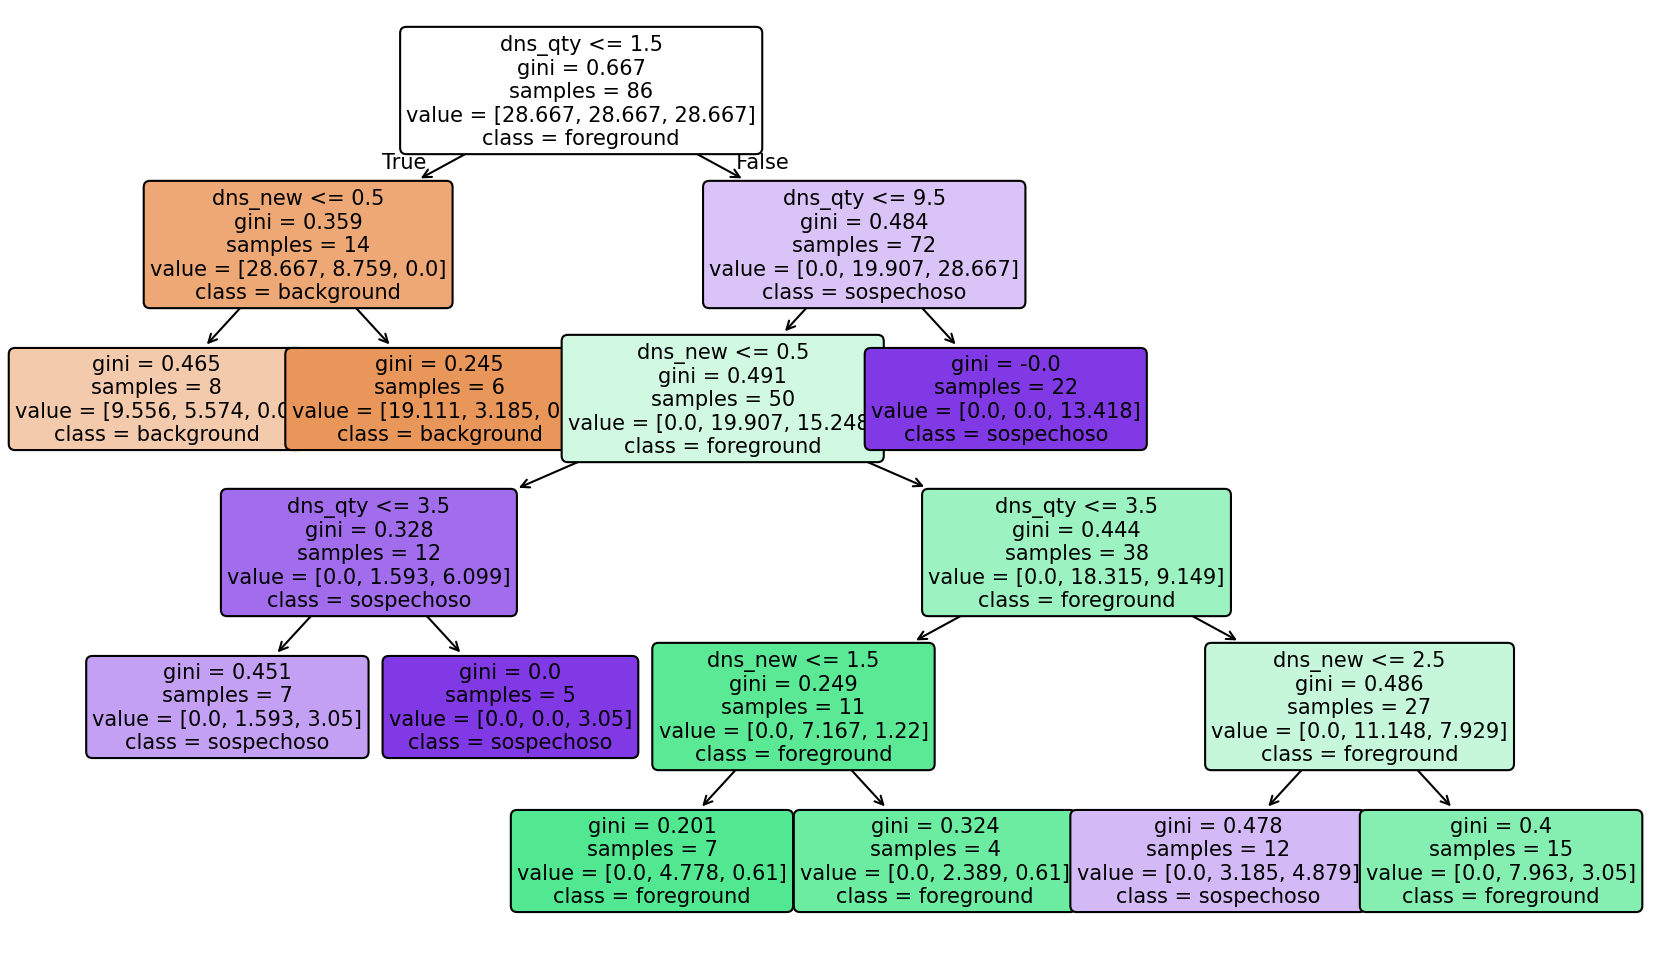
\includegraphics[width=\textwidth]{graficas/arbol_decision.png}
\caption{Árbol de decisión entrenado}
\label{fig:arbol}
\end{figure}

La lógica de decisión es la siguiente:

\begin{itemize}
    \item \textbf{dns\_qty $\leq$ 1.5} $\rightarrow$ Background (tráfico de fondo mínimo)
    \item \textbf{1.5 $<$ dns\_qty $\leq$ 9.5} $\rightarrow$ Depende de dns\_new:
        \begin{itemize}
            \item \textbf{dns\_new $\leq$ 0.5} y \textbf{dns\_qty $\leq$ 3.5} $\rightarrow$ Sospechoso
            \item \textbf{dns\_new $\leq$ 0.5} y \textbf{dns\_qty $>$ 3.5} $\rightarrow$ Sospechoso
            \item \textbf{dns\_new $>$ 0.5} y \textbf{dns\_qty $\leq$ 3.5} $\rightarrow$ Foreground
            \item \textbf{dns\_new $>$ 0.5} y \textbf{dns\_qty $>$ 3.5} $\rightarrow$ Foreground o Sospechoso según dns\_new
        \end{itemize}
    \item \textbf{dns\_qty $>$ 9.5} $\rightarrow$ Sospechoso (pico anómalo)
\end{itemize}

\subsection{Recursos del sistema}
\label{sec:recursos}

\begin{table}[H]
\centering
\caption{Consumo de recursos del ESP32}
\label{tab:recursos}
\begin{tabular}{lrr}
\toprule
\textbf{Recurso} & \textbf{Usado} & \textbf{Disponible} \\
\midrule
Flash (programa) & 756,037 bytes (57.7\%) & 1,310,720 bytes \\
RAM (datos)      & 73,364 bytes (22.4\%) & 327,680 bytes \\
\bottomrule
\end{tabular}
\end{table}

El árbol de decisión ocupa aproximadamente 130 bytes en flash (13 nodos $\times$ 10 bytes cada uno). La latencia de inferencia es menor a 1 microsegundo.

% =====================================================================
% g) INFORME COMPLETO Y PROTOTIPO FUNCIONANDO
% =====================================================================
\section{Prototipo Funcionando}
\label{sec:prototipo}

\subsection{Despliegue}
\label{sec:despliegue}

El prototipo se desplegó en la siguiente configuración:

\begin{itemize}
    \item \textbf{ESP32} conectado a internet via WiFi (STA).
    \item Red local \texttt{ESP32-Monitor} disponible para clientes.
    \item NAPT habilitado: los clientes del AP tienen internet.
    \item Servidor EC2 en \texttt{18.116.200.170} corriendo:
        \begin{itemize}
            \item \texttt{csi\_ws.py}: WebSocket broker (puerto 3001) + HTTP POST (puerto 3002)
            \item Apache2: sirve \texttt{dns.html} en \texttt{/var/www/html/}
        \end{itemize}
\end{itemize}

\subsection{Dashboard web}
\label{sec:dashboard}

El dashboard se accede en \texttt{http://18.116.200.170/dns.html}. Muestra:

\begin{itemize}
    \item \textbf{Badge en tiempo real} de la clasificación actual (bg/fg/sos)
    \item \textbf{Métricas numéricas}: dns\_qty, dns\_unique, dns\_new, score de anomalía
    \item \textbf{Gráfico de líneas}: evolución de las 3 features en el tiempo
    \item \textbf{Gráfico circular}: distribución de clases
    \item \textbf{Timeline}: historial de clasificaciones
\end{itemize}

\begin{figure}[H]
\centering
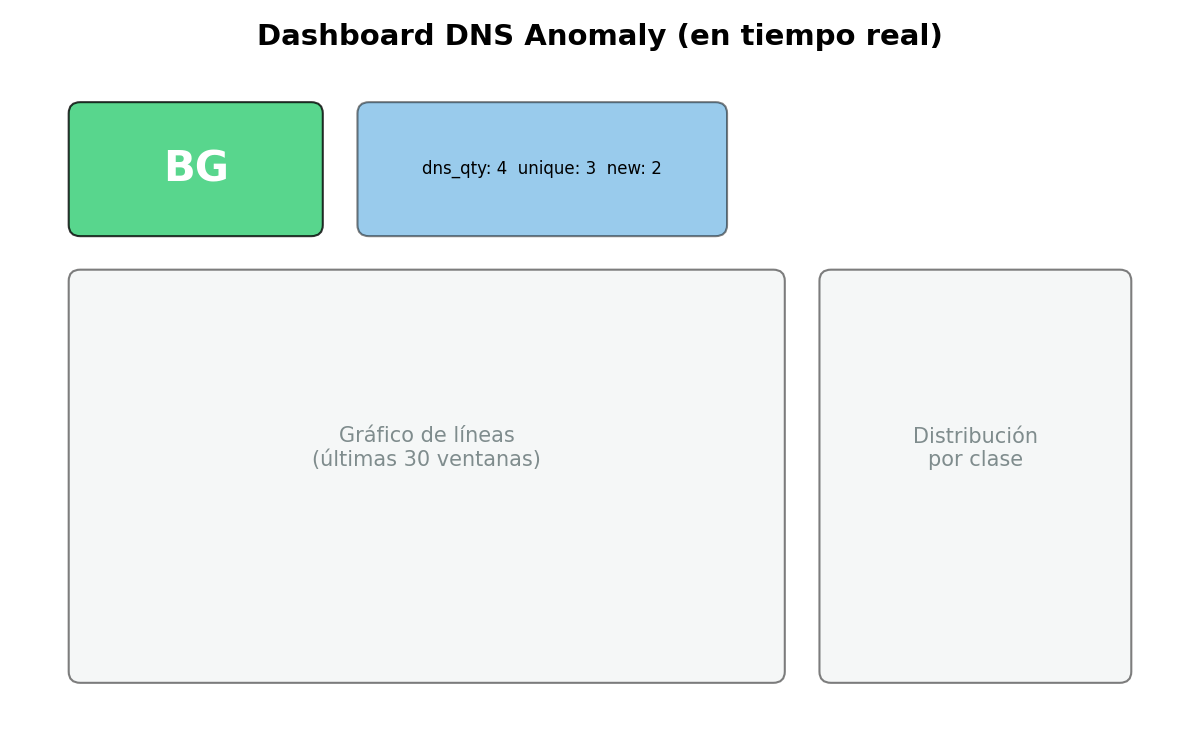
\includegraphics[width=\textwidth]{graficas/dashboard.png}
\caption{Dashboard web en tiempo real (dns.html)}
\label{fig:dashboard}
\end{figure}

\subsection{Validación}
\label{sec:validacion}

Se realizaron las siguientes pruebas:

\begin{enumerate}
    \item \textbf{NAPT:} Teléfono conectado al AP del ESP32 con datos móviles apagados. Verificación de que puede navegar por internet.
    \item \textbf{Clasificación:} Navegación activa (YouTube, Google, Facebook) produce clasificación \texttt{fg}. Reposo produce \texttt{bg}. Escaneo de puertos produce \texttt{sos}.
    \item \textbf{Dashboard:} Los datos aparecen en el dashboard web con latencia menor a 1 segundo.
\end{enumerate}

\subsection{Discusión}
\label{sec:discusion}

La precisión del 64.86\% es modesta pero esperable dado el desbalance de clases (solo 4 muestras de background). Las principales limitaciones son:

\begin{itemize}
    \item \textbf{Pocas muestras de background:} El tráfico de fondo es difícil de capturar porque el ESP32 mismo genera consultas DNS.
    \item \textbf{3 features solamente:} Agregar features como TTL, tamaños de paquete o tiempos de respuesta podría mejorar la precisión.
    \item \textbf{Árbol poco profundo:} Un modelo más complejo (Random Forest o MLP cuantizado) podría dar mejor precisión, pero ocuparía más recursos.
\end{itemize}

% =====================================================================
% CONCLUSIONES
% =====================================================================
\section{Conclusiones}
\label{sec:conclusiones}

Se implementó un sistema de detección de anomalías DNS en tiempo real utilizando TinyML en un ESP32, cumpliendo los objetivos planteados:

\begin{enumerate}
    \item El forwarder DNS captura y reenvía consultas correctamente.
    \item Las ventanas de 3s permiten extraer features significativas.
    \item El árbol de decisión clasifica con 64.86\% de precisión.
    \item La inferencia en ESP32 es prácticamente instantánea ($\ll$1 ms).
    \item El dashboard web muestra los resultados en tiempo real.
    \item El prototipo funciona con tráfico real de navegación.
\end{enumerate}

La hipótesis H1 se confirma parcialmente: las 3 features DNS permiten distinguir entre clases, pero con margen de mejora. H2 se confirma: el árbol ocupa menos de 200 bytes y la inferencia es insignificante. H3 se confirma: la precisión supera el 60\% con solo 3 features.

\subsection{Trabajo futuro}
\label{sec:futuro}

\begin{itemize}
    \item Balancear el dataset con más muestras de background.
    \item Probar modelos más complejos (Random Forest, MLP cuantizado).
    \item Agregar más features (longitud de nombres, TTL, tipos de registro).
    \item Implementar aprendizaje联邦ado entre múltiples ESP32.
    \item Mejorar el dashboard con alertas y notificaciones.
\end{itemize}

% ---- Bibliografía ----
\begin{thebibliography}{99}

\bibitem{patnaik2026tinyml}
P.~Patnaik, S.~Mishra, B.~Panda, and S.~K.~Kar,
``TinyML Driven Intrusion Detection for 5G Network Slices with Leakage-Free Validation,''
\textit{Next-Generation Computing Systems and Technologies}, vol.~2, no.~1, pp.~10--20, 2026.

\bibitem{stacking2025tinyml}
``An optimized stacking-based TinyML model for attack detection in IoT networks,''
\textit{PLOS One}, Aug.~2025.

\bibitem{anand2026energy}
A.~Parmar and K.~Borisagar,
``Energy-Aware Federated TinyML for Anomaly Detection over LoRaWAN,''
\textit{IJCRT}, vol.~14, no.~4, Apr.~2026.

\bibitem{nassef2026lightweight}
L.~Nassef \textit{et al.},
``Lightweight and Energy-Aware Intrusion Detection for Industrial IoT Using TinyML and Edge AI,''
\textit{Scientific Reports}, vol.~16, p.~18524, 2026.

\bibitem{esp32tinyml}
``Efficient Machine Learning Models for Intrusion Detection on ESP32,''
(manuscrito en preparación).

\end{thebibliography}

\end{document}
